\documentclass[11pt]{preprint}

\setlength{\topmargin}{0mm} \setlength{\oddsidemargin}{0mm}
\setlength{\textwidth}{160mm} \setlength{\textheight}{215mm}

\usepackage{amssymb,amsmath,amscd,amsthm}
\usepackage{graphics}
\usepackage{tikz}

\def\enumb{\begin{enumerate}}
\def\enume{\end{enumerate}}
\def\itemb{\begin{itemize}}
\def\iteme{\end{itemize}}
\def\integers{\mathbb{Z}}

\def\multiset#1#2{\ensuremath{\left(\kern-.3em\left(\genfrac{}{}{0pt}{}{#1}{#2}\right)\kern-.3em\right)}}



\newtheorem{proposition}{Proposition}
\newtheorem{theorem}{Theorem}

\title{Discrete Mathematics, 2016 Fall - Worksheet 24}
\author{Instructor: Zsolt Pajor-Gyulai, CIMS}



\begin{document}

\maketitle

In all of the above problems explain your answer in full English sentences.

\enumb
\item For which values of $n$ is the complete graph $K_n$ Eulerian?

We know that the complete graph $K_n$ is $n-1$ regular and therefore every edge will have an even degree (and be therefore Eulerian) if an only if $n$ is odd. 
\item Let $G$ be a connected graph that is not Eulerian. Prove that it is possible to add a single vertex to $G$, together with some edges from this new vertex to some old vertices such that the new graph is Eulerian.

\begin{proof}
Connect the two vertex into every vertex of $G$ with an odd degree. Then all vertices of the new graph have an even degree except perhaps the new vertex. However, this last vertex must have an even degree as well, otherwise the sum of all the degrees would not add up to an even number. Therefore all degrees in the new graph have an even degree and therefore the new graph is Eulerian.
\end{proof}

\item Let $G$ be the graph in the following figure.
\begin{figure}[ht]
\centering
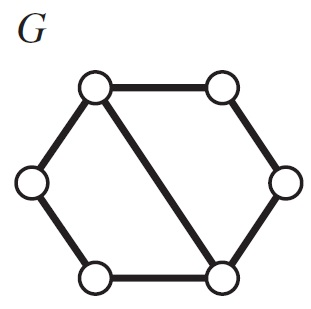
\includegraphics[scale=0.5]{Color1.jpg}
\end{figure}
Please find $\chi(G)$.

Note that this graph contains no odd cycles and therefore $\chi(G)=2$, i.e. it is bipartite.

\item Let $G$ be a graph and let $v$ be a vertex of $G$. Prove that
\[
\chi(G-v)\leq \chi(G)\leq \chi(G-v)+1
\]
\begin{proof}
The first inequality follows immediately as $G-v$ is a subgraph of $G$.  To see the other one, let $f$ be a proper coloring of $G-v$. Then assigning the same colors in $G$ and a completely new color assigned to $v$ gives a coloring of $G$ with $\chi(G-v)+1$ colors.
\end{proof}
\item Let $G=K_{n,m}$. Determine $|V(G)|$ and $|E(G)|$.

Clearly, $|V(G)|=n+m$. Since there is an edge between all vertices belonging to different parts, $|E(G)|=nm$.

\item Let $G$ be a graph with $n$ vertices. Prove that $\chi(G)\chi(\bar{G})\geq n$.

\begin{proof}
Let $f$ be a proper $\chi(G)$ coloring of $G$  and $g$ be a proper $\chi(\bar{G})$ coloring of $\bar{G}$ Let
\[
n_i=|\{v\in V(G): f(v)=i\},
\]
i.e. the number of vertices that are assigned the $i$th color. Then clearly
\[
n=\sum_{i=1}^{\chi(G)}n_i\leq \chi(G)\cdot \max_{i=1,\dots,\chi(G)}{n}_i.
\]
If two vertices in $V(G)$ are assigned the same color, then they are not adjacent in $G$ and therefore they are adjacent in $\bar{G}$ and therefore they are assigned different colors under $g$. This implies
\[
n_i \leq \chi(\bar{G}),\qquad\forall i=1,\dots,\chi(G).
\]
Putting the previous two displays together, we get
\[
n\leq \chi(G)\cdot \max_{i=1,\dots,\chi(G)}{n}_i\leq \chi(G)\chi(\bar{G})
\]
\end{proof}
\enume
\end{document}